\subsection{Benchmark Overview}
We compare Approximate Convex Decomposition (ACD) and Visibility Clique Cover
(VCC) within an otherwise identical GCS--B\'ezier planning pipeline. The
benchmark comprises five structured map families---\code{clustered},
\code{narrows}, \code{rooms}, \code{u\_shaped}, and \code{flappy}---with ten
independently generated geometries per family. All geometries use a workspace
scale of $L=5$, dense obstacle placement, medium obstacle size, and
area-coverage generation. ACD is deterministic under the fixed configuration
and is run once per geometry. To expose the stochastic variability of the
visibility sampling and clique cover, VCC is run with ten decomposition seeds
per geometry. The resulting evaluation contains 50 ACD runs and 500 VCC trials;
all method comparisons use the geometry, rather than the VCC trial, as the
independent unit of analysis.

ACD produced a valid trajectory on all 50 geometries. VCC succeeded in 489 of
500 trials: 100/100 on \code{clustered} and \code{u\_shaped}, 98/100 on
\code{flappy}, 96/100 on \code{rooms}, and 95/100 on \code{narrows}. Every
geometry had at least one successful VCC trial, but the within-geometry success
rate fell to 0.70 on \code{narrows} seed~3 and to 0.90 on \code{narrows}
seeds~1 and~8. These outcomes show that a single successful VCC realization
does not characterize robustness in a narrow-passage environment.

The available summary records localize, but do not uniquely classify, the VCC
failures. All ten trials for the affected \code{narrows} geometries contain
decomposition time, region and edge counts, visible-edge counts, clique counts,
and coverage estimates. A region graph was therefore constructed before the
unsuccessful trials terminated, which is inconsistent with a failure that
simply produced no clique cover. The summaries do not retain the raw
\code{stage}, \code{decomp\_failed\_reason}, or \code{error\_message} fields
needed to distinguish graph disconnection from a solver or trajectory-certificate
failure. A technically plausible explanation is that stochastic visibility
sampling attains high global coverage while failing to generate an overlapping
bridge through one mandatory narrow gate; this can isolate the start- and
goal-connected subgraphs even when total region and edge counts appear
unexceptional. This mechanism is a hypothesis to be tested from the raw failure
logs, not a failure label inferred from aggregate counts.

\subsection{Model Size and Runtime}
Table~\ref{tab:exp-runtime} reports the median and IQR of the ten geometry-level values
in each family. For VCC, each geometry-level value is itself the median over its
ten trials; failed trials remain in the success endpoint and are excluded only
from trajectory-dependent quantities. Across-geometry interquartile ranges
(IQRs) are reported in the text to expose dispersion without treating repeated
VCC trials on the same geometry as independent observations.

\begin{table}[htbp]
\caption{Model size and runtime by map family, reported as median [Q1, Q3] across ten geometries. For VCC, each geometry contributes its median over ten trials. Time is measured in seconds.}
\label{tab:exp-runtime}
\centering
\scriptsize
\setlength{\tabcolsep}{2.2pt}
\resizebox{\textwidth}{!}{%
\begin{tabular}{@{}llrrrrrr@{}}
\toprule
Map & Method & Success & $N_R$ & $N_E$ & $t_{\rm dec}$ & $t_{\rm solve}$ & $t_{\rm e2e}$ \\
\midrule
Clustered & ACD & 10/10 & 188 [185.5,189.8] & 433 [422.3,449.3] & 15.48 [14.75,16.27] & 102.63 [97.26,128.64] & 117.52 [112.45,145.62] \\
          & VCC & 100/100 & 34.5 [33.1,35.4] & 50 [47.6,55.4] & 137.70 [134.41,142.56] & 3.74 [3.04,4.27] & 141.61 [138.22,145.50] \\
Narrows   & ACD & 10/10 & 15 [15,15] & 21 [20.3,22] & 0.83 [0.82,0.87] & 1.01 [0.79,1.15] & 1.84 [1.64,1.98] \\
          & VCC & 95/100 & 17.3 [15.8,18.6] & 37.3 [32.0,46.1] & 18.87 [18.26,19.75] & 2.28 [2.10,2.66] & 21.38 [20.22,22.52] \\
Rooms     & ACD & 10/10 & 31 [29.5,31] & 52 [48.3,52] & 1.64 [1.54,1.76] & 3.78 [3.08,4.60] & 5.43 [4.69,6.38] \\
          & VCC & 96/100 & 14 [14,14] & 16.8 [16.1,19.4] & 18.07 [17.40,18.52] & 0.48 [0.43,0.67] & 18.62 [17.75,19.02] \\
U-shaped  & ACD & 10/10 & 21.5 [20.0,22.8] & 32.5 [29.5,35.5] & 1.08 [1.03,1.14] & 1.53 [1.23,1.88] & 2.63 [2.25,2.94] \\
          & VCC & 100/100 & 15.5 [15,16] & 43.3 [39.0,46.4] & 14.84 [14.00,14.98] & 2.95 [2.36,3.55] & 17.43 [17.06,18.23] \\
Flappy    & ACD & 10/10 & 25 [25,25] & 24 [24,24] & 1.80 [1.78,1.84] & 0.29 [0.28,0.29] & 2.08 [2.07,2.13] \\
          & VCC & 98/100 & 25 [25,25] & 24 [24,24] & 21.56 [21.43,21.80] & 0.33 [0.32,0.35] & 21.87 [21.75,22.19] \\
\bottomrule
\end{tabular}
}
\end{table}

VCC most strongly compresses the \code{clustered} graphs: relative to ACD, it
reduces the median region count from 188 to 34.5, the median edge count from 433
to 50, and the median GCS time from 102.63~s to 3.74~s. This reduction is stable
across geometries: the IQRs are $[185.5,189.8]$ versus $[33.1,35.4]$ regions
and $[422.3,449.3]$ versus $[47.6,55.4]$ edges for ACD and VCC, respectively.
Nevertheless, VCC decomposition requires 137.70~s (IQR
$[134.41,142.56]$~s), so its median end-to-end time remains 24.09~s higher.
The result isolates the trade-off: VCC creates a substantially cheaper online
optimization problem, but its offline construction cost dominates a single
query.

Graph compression is topology dependent rather than a necessary consequence of
using fewer regions. On \code{u\_shaped}, VCC reduces the median region count
from 21.5 to 15.5 yet increases the edge count from 32.5 to 43.3 and the GCS
time from 1.53~s to 2.95~s. Conversely, on \code{rooms}, VCC reduces both the
edge count (52 to 16.8) and GCS time (3.78~s to 0.48~s). These contrasting cases
show that region aggregation is computationally useful only when it also
controls the intersection structure of the induced graph.

Across all 50 paired geometries, two-sided Wilcoxon signed-rank tests with Holm
correction over six prespecified comparisons confirm higher VCC decomposition
cost ($p_{\rm adj}<1.1\times10^{-14}$), fewer VCC regions
($p_{\rm adj}<9.3\times10^{-6}$), and a method difference in edge count
($p_{\rm adj}=0.019$). The apparent difference in GCS time is not significant
after correction ($p_{\rm raw}=0.048$, $p_{\rm adj}=0.097$), reflecting the
opposing family-specific effects above. End-to-end time favors ACD in every map
family: its IQR is $[112.45,145.62]$~s on \code{clustered} and remains below
6.38~s at the upper quartile in each other family, whereas VCC's family-level
median is at least 17.43~s outside \code{clustered}. Thus, ACD is the appropriate
default for a single query under this protocol.

Table~\ref{tab:exp-significance} reports the complete test statistics. We use
the Wilcoxon signed-rank test because ACD and VCC are evaluated on the same
geometries; an unpaired Mann--Whitney U test would discard this pairing and is
therefore inappropriate here. Differences are defined as the ACD value minus
the geometry-level VCC median. Holm adjustment controls the family-wise error
rate across the six comparisons at $\alpha=0.05$.

\begin{table}[htbp]
\caption{Paired two-sided Wilcoxon signed-rank tests over 50 geometries. $\widetilde{\Delta}$ is the median paired difference (ACD minus VCC).}
\label{tab:exp-significance}
\centering
\scriptsize
\setlength{\tabcolsep}{4.0pt}
\begin{tabular}{@{}lrrrrl@{}}
\toprule
Metric & $n$ & $\widetilde{\Delta}$ & $W$ & $p_{\rm raw}$ & $p_{\rm Holm}$ \\
\midrule
$t_{\rm dec}$       & 50 & $-18.539$ & 0     & $1.78\times10^{-15}$ & $1.07\times10^{-14}$ \\
$t_{\rm solve}$     & 50 & $-0.032$  & 433   & 0.0483 & 0.0966 \\
$N_R$                & 50 & $6.5$     & 71    & $1.95\times10^{-6}$ & $9.30\times10^{-6}$ \\
$N_E$                & 50 & $0.0$     & 233.5 & 0.0064 & 0.0192 \\
Path length          & 50 & $-0.144$  & 541   & 0.3572 & 0.3572 \\
Minimum clearance    & 50 & $-0.00239$& 174   & $1.86\times10^{-6}$ & $9.30\times10^{-6}$ \\
\bottomrule
\end{tabular}
\end{table}

\subsection{Correlation Between Model Size and Solve Time}
Figure~\ref{fig:exp-correlations} relates graph size to solve time using the
current benchmark summaries. Each of the 100 observations represents one
method--geometry pair: the single ACD run or the median of the ten VCC trials on
that geometry. Edge count is substantially more strongly associated with solve
time than region count. The Spearman coefficients are $\rho=0.884$
($p=4.34\times10^{-34}$) for $N_E$ and $\rho=0.514$
($p=4.59\times10^{-8}$) for $N_R$. Both associations are statistically
detectable, but their magnitudes differ considerably.

\begin{figure}[h!]
\centering
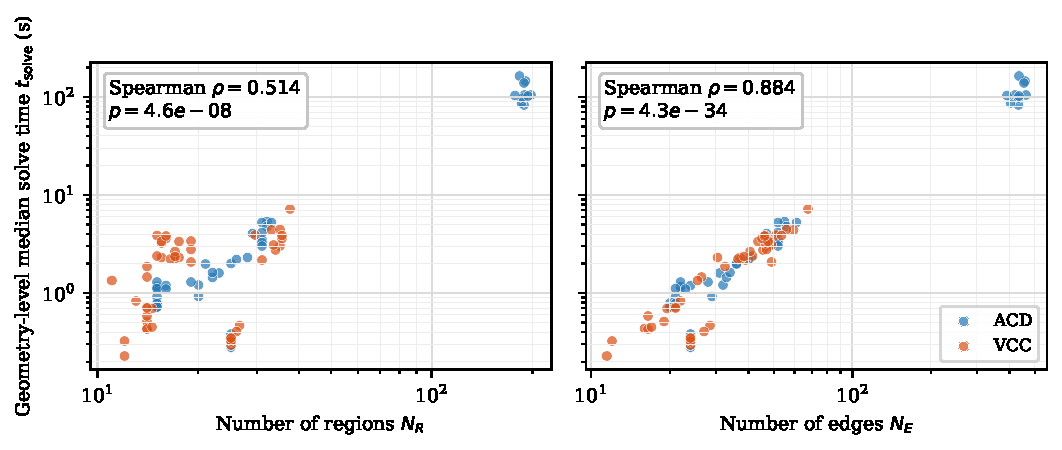
\includegraphics[width=\textwidth]{5-Experimental-results/figures/correlation_geometry_level.pdf}
\caption{Geometry-level relationships between graph size and solve time in the current benchmark ($n=100$ method--geometry observations). VCC contributes its within-geometry median over ten trials. Both axes are logarithmic; colors distinguish the decomposition methods. Reported coefficients and $p$-values are from two-sided Spearman rank-correlation tests.}
\label{fig:exp-correlations}
\end{figure}

This disparity follows from how a GCS program is assembled. A region contributes
a local copy of the continuous state and its within-set constraints, but each
directed edge introduces a flow variable together with edge-conditioned copies
of endpoint variables. For a B\'ezier trajectory, these copies are
high-dimensional because they carry control points and timing variables, and
their activation requires perspective formulations of continuity, derivative,
and cost constraints. Increasing $N_E$ therefore expands several coupled blocks
of variables and conic constraints per adjacency, not merely a scalar incidence
matrix. A dense graph also gives presolve more candidate flows and bounds to
propagate, weakens simple topological pruning when many alternate routes remain,
and enlarges the relaxation subsequently passed to rounding. The stronger
edge-count association is consequently consistent with $N_E$ acting as a
pre-construction proxy for this edge-bound algebraic workload, whereas $N_R$
does not encode how densely the regions intersect. Correlation alone does not
establish a causal scaling law, and the observations are pooled across map
families and methods; nevertheless, the formulation explains why
decompositions with similar $N_R$ can have markedly different solve times.

\subsection{Trajectory Quality}
Table~\ref{tab:exp-quality} reports trajectory medians and IQRs using the same
geometry-level aggregation. Path length does not identify a uniform winner:
the across-geometry paired median difference (ACD minus VCC) is $-0.144$, and a
two-sided Wilcoxon test provides no evidence of a method effect
($p_{\rm adj}=0.357$). The family-level differences are small on
\code{flappy} and \code{narrows}, favor VCC on \code{rooms}, and favor ACD on
\code{clustered} and \code{u\_shaped}.

\begin{table}[htbp]
\caption{Trajectory-quality metrics reported as median [Q1, Q3] across ten geometries. Failed trials are excluded from trajectory-dependent summaries.}
\label{tab:exp-quality}
\centering
\scriptsize
\setlength{\tabcolsep}{2.5pt}
\resizebox{\textwidth}{!}{%
\begin{tabular}{@{}llrrrr@{}}
\toprule
Map & Method & Path length & Traj. time & Min. clearance & Active regions \\
\midrule
Clustered & ACD & 7.62 [7.41,7.98] & 9.90 [9.78,10.48] & $7.43{\times}10^{-5}$ [$4.33{\times}10^{-5}$,$1.60{\times}10^{-4}$] & 16 [15,17.8] \\
          & VCC & 8.52 [8.46,8.60] & 8.91 [8.62,9.14] & $8.44{\times}10^{-2}$ [$5.92{\times}10^{-2}$,$1.54{\times}10^{-1}$] & 5.5 [4.3,6.8] \\
Narrows   & ACD & 16.35 [15.86,17.32] & 24.05 [23.90,24.43] & $3.66{\times}10^{-4}$ [$1.19{\times}10^{-4}$,$4.89{\times}10^{-4}$] & 13 [11.5,13.8] \\
          & VCC & 16.14 [15.76,16.35] & 25.87 [24.32,26.80] & $1.08{\times}10^{-3}$ [$7.05{\times}10^{-4}$,$1.65{\times}10^{-3}$] & 9 [9,9] \\
Rooms     & ACD & 7.55 [7.48,7.59] & 8.53 [8.19,8.68] & $1.06{\times}10^{-3}$ [$2.88{\times}10^{-4}$,$4.80{\times}10^{-3}$] & 11 [11,11.8] \\
          & VCC & 7.16 [7.16,7.26] & 7.03 [7.02,7.06] & $4.51{\times}10^{-3}$ [$3.41{\times}10^{-3}$,$5.31{\times}10^{-3}$] & 7 [7,7.5] \\
U-shaped  & ACD & 7.61 [7.55,8.00] & 7.96 [7.57,8.30] & $6.89{\times}10^{-4}$ [$3.03{\times}10^{-4}$,$1.58{\times}10^{-3}$] & 8 [7,9] \\
          & VCC & 8.10 [7.85,8.30] & 8.22 [8.06,8.38] & $2.11{\times}10^{-2}$ [$1.13{\times}10^{-2}$,$3.57{\times}10^{-2}$] & 5 [5,5.5] \\
Flappy    & ACD & 52.65 [52.56,52.76] & 71.32 [70.91,71.91] & $2.09{\times}10^{-4}$ [$7.98{\times}10^{-5}$,$4.45{\times}10^{-4}$] & 23 [23,23] \\
          & VCC & 52.81 [52.79,52.97] & 71.15 [70.76,71.50] & $2.49{\times}10^{-4}$ [$1.34{\times}10^{-4}$,$5.37{\times}10^{-4}$] & 25 [25,25] \\
\bottomrule
\end{tabular}
}
\end{table}

VCC has higher median minimum clearance in every family. The paired comparison
is significant after Holm correction ($p_{\rm adj}<9.3\times10^{-6}$), but the
effect is heterogeneous: VCC's clearance IQR is
$[5.92\times10^{-2},1.54\times10^{-1}]$ on \code{clustered} and
$[1.13\times10^{-2},3.57\times10^{-2}]$ on \code{u\_shaped}, compared with
$[1.34\times10^{-4},5.37\times10^{-4}]$ on \code{flappy}. The visibility cover
can therefore bias the optimizer toward routes supported by larger overlapping
free-space sets, but it does not impose a clearance objective and should not be
interpreted as a safety guarantee. Moreover, the clearance gain coexists with
higher decomposition time and reduced stochastic reliability in constrained
families. This is a Pareto trade-off rather than evidence that either
decomposition dominates in trajectory quality.

Relaxation behavior provides a second distinction. The corridor-like graphs in
the \code{flappy} family admit few meaningful route alternatives, so their relaxed
and rounded objectives remain close. In more highly connected
\code{clustered} graphs, fractional flow can distribute over competing routes,
increasing the relaxation--rounding gap even after VCC reduces graph size.
Hence, graph compactness, relaxation tightness, and geometric clearance are
related but non-equivalent properties of a decomposition.

\subsection{Visual Evidence on Flappy Maps}
The \code{flappy} family provides a qualitative stress test because every route
must alternate between upper and lower openings. Figure~\ref{fig:exp-flappy}
shows four representative geometries. Both decompositions preserve the
mandatory corridor sequence, consistent with their nearly equal median path
lengths (52.65 for ACD and 52.81 for VCC) and traversal times (71.32~s and
71.15~s). The images therefore corroborate geometric feasibility and route
similarity, but they do not establish statistical equivalence.

\begin{figure}[htbp]
\centering
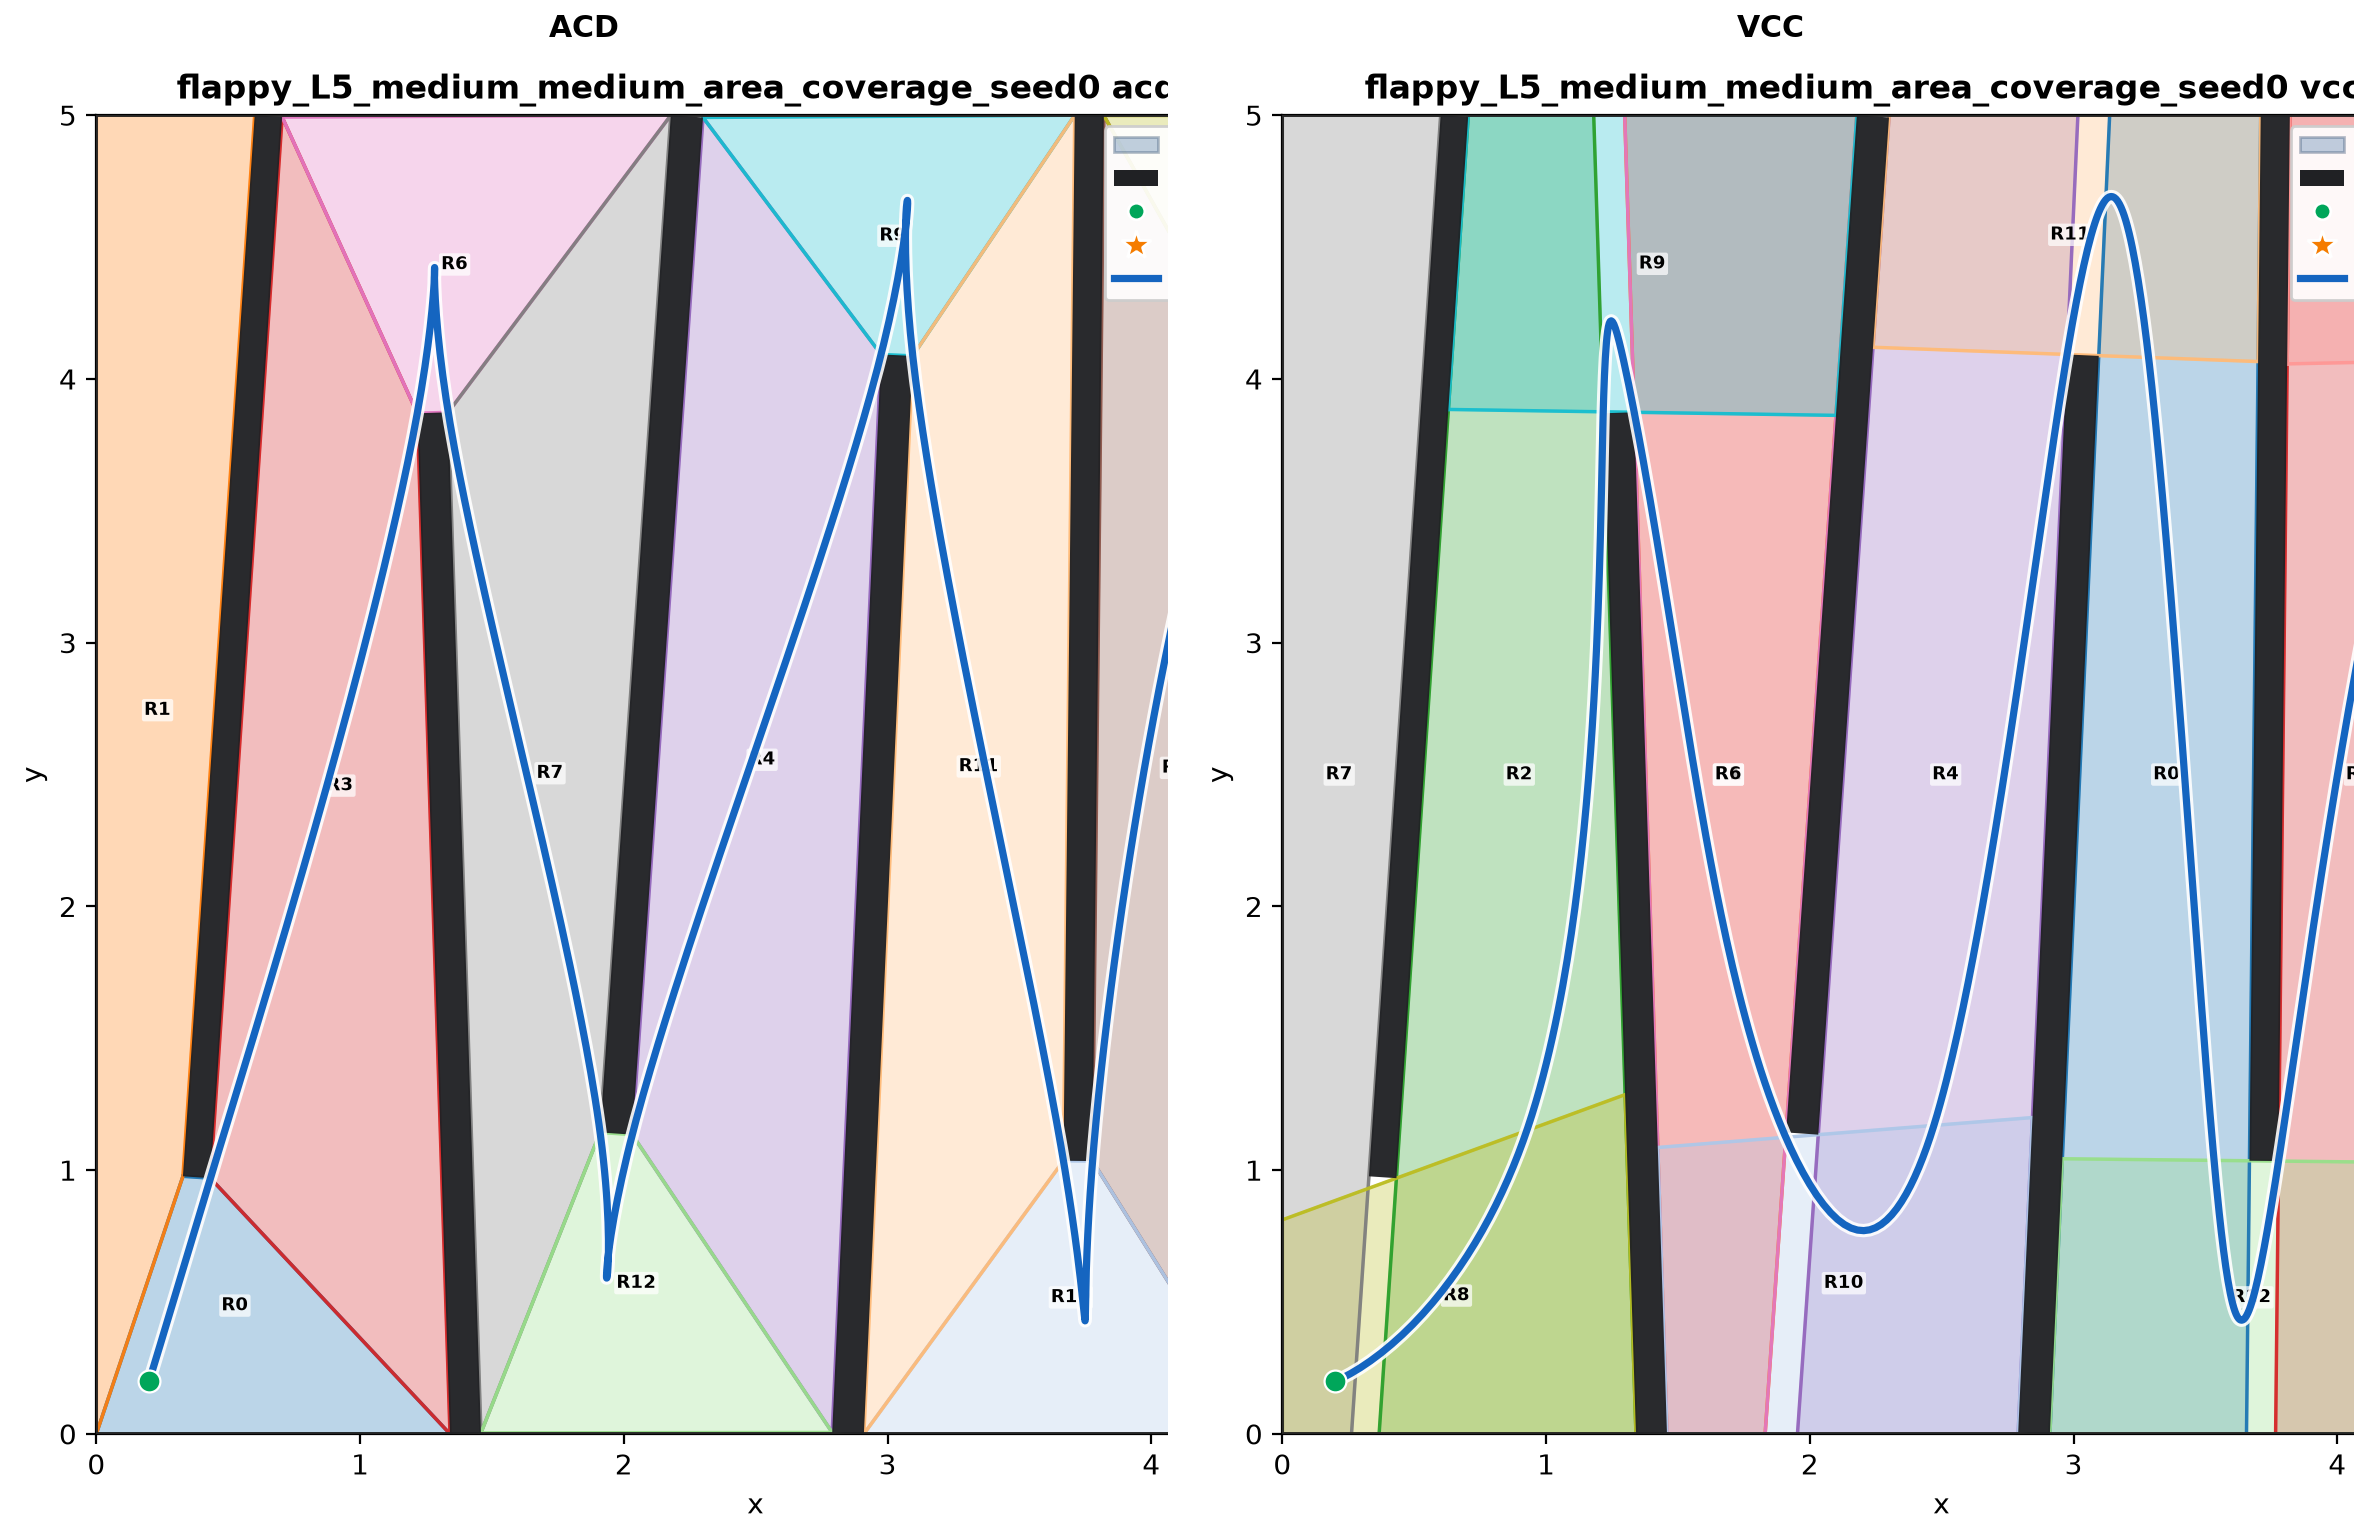
\includegraphics[width=0.48\textwidth]{5-Experimental-results/figures/flappy_seed0_comparison.png}
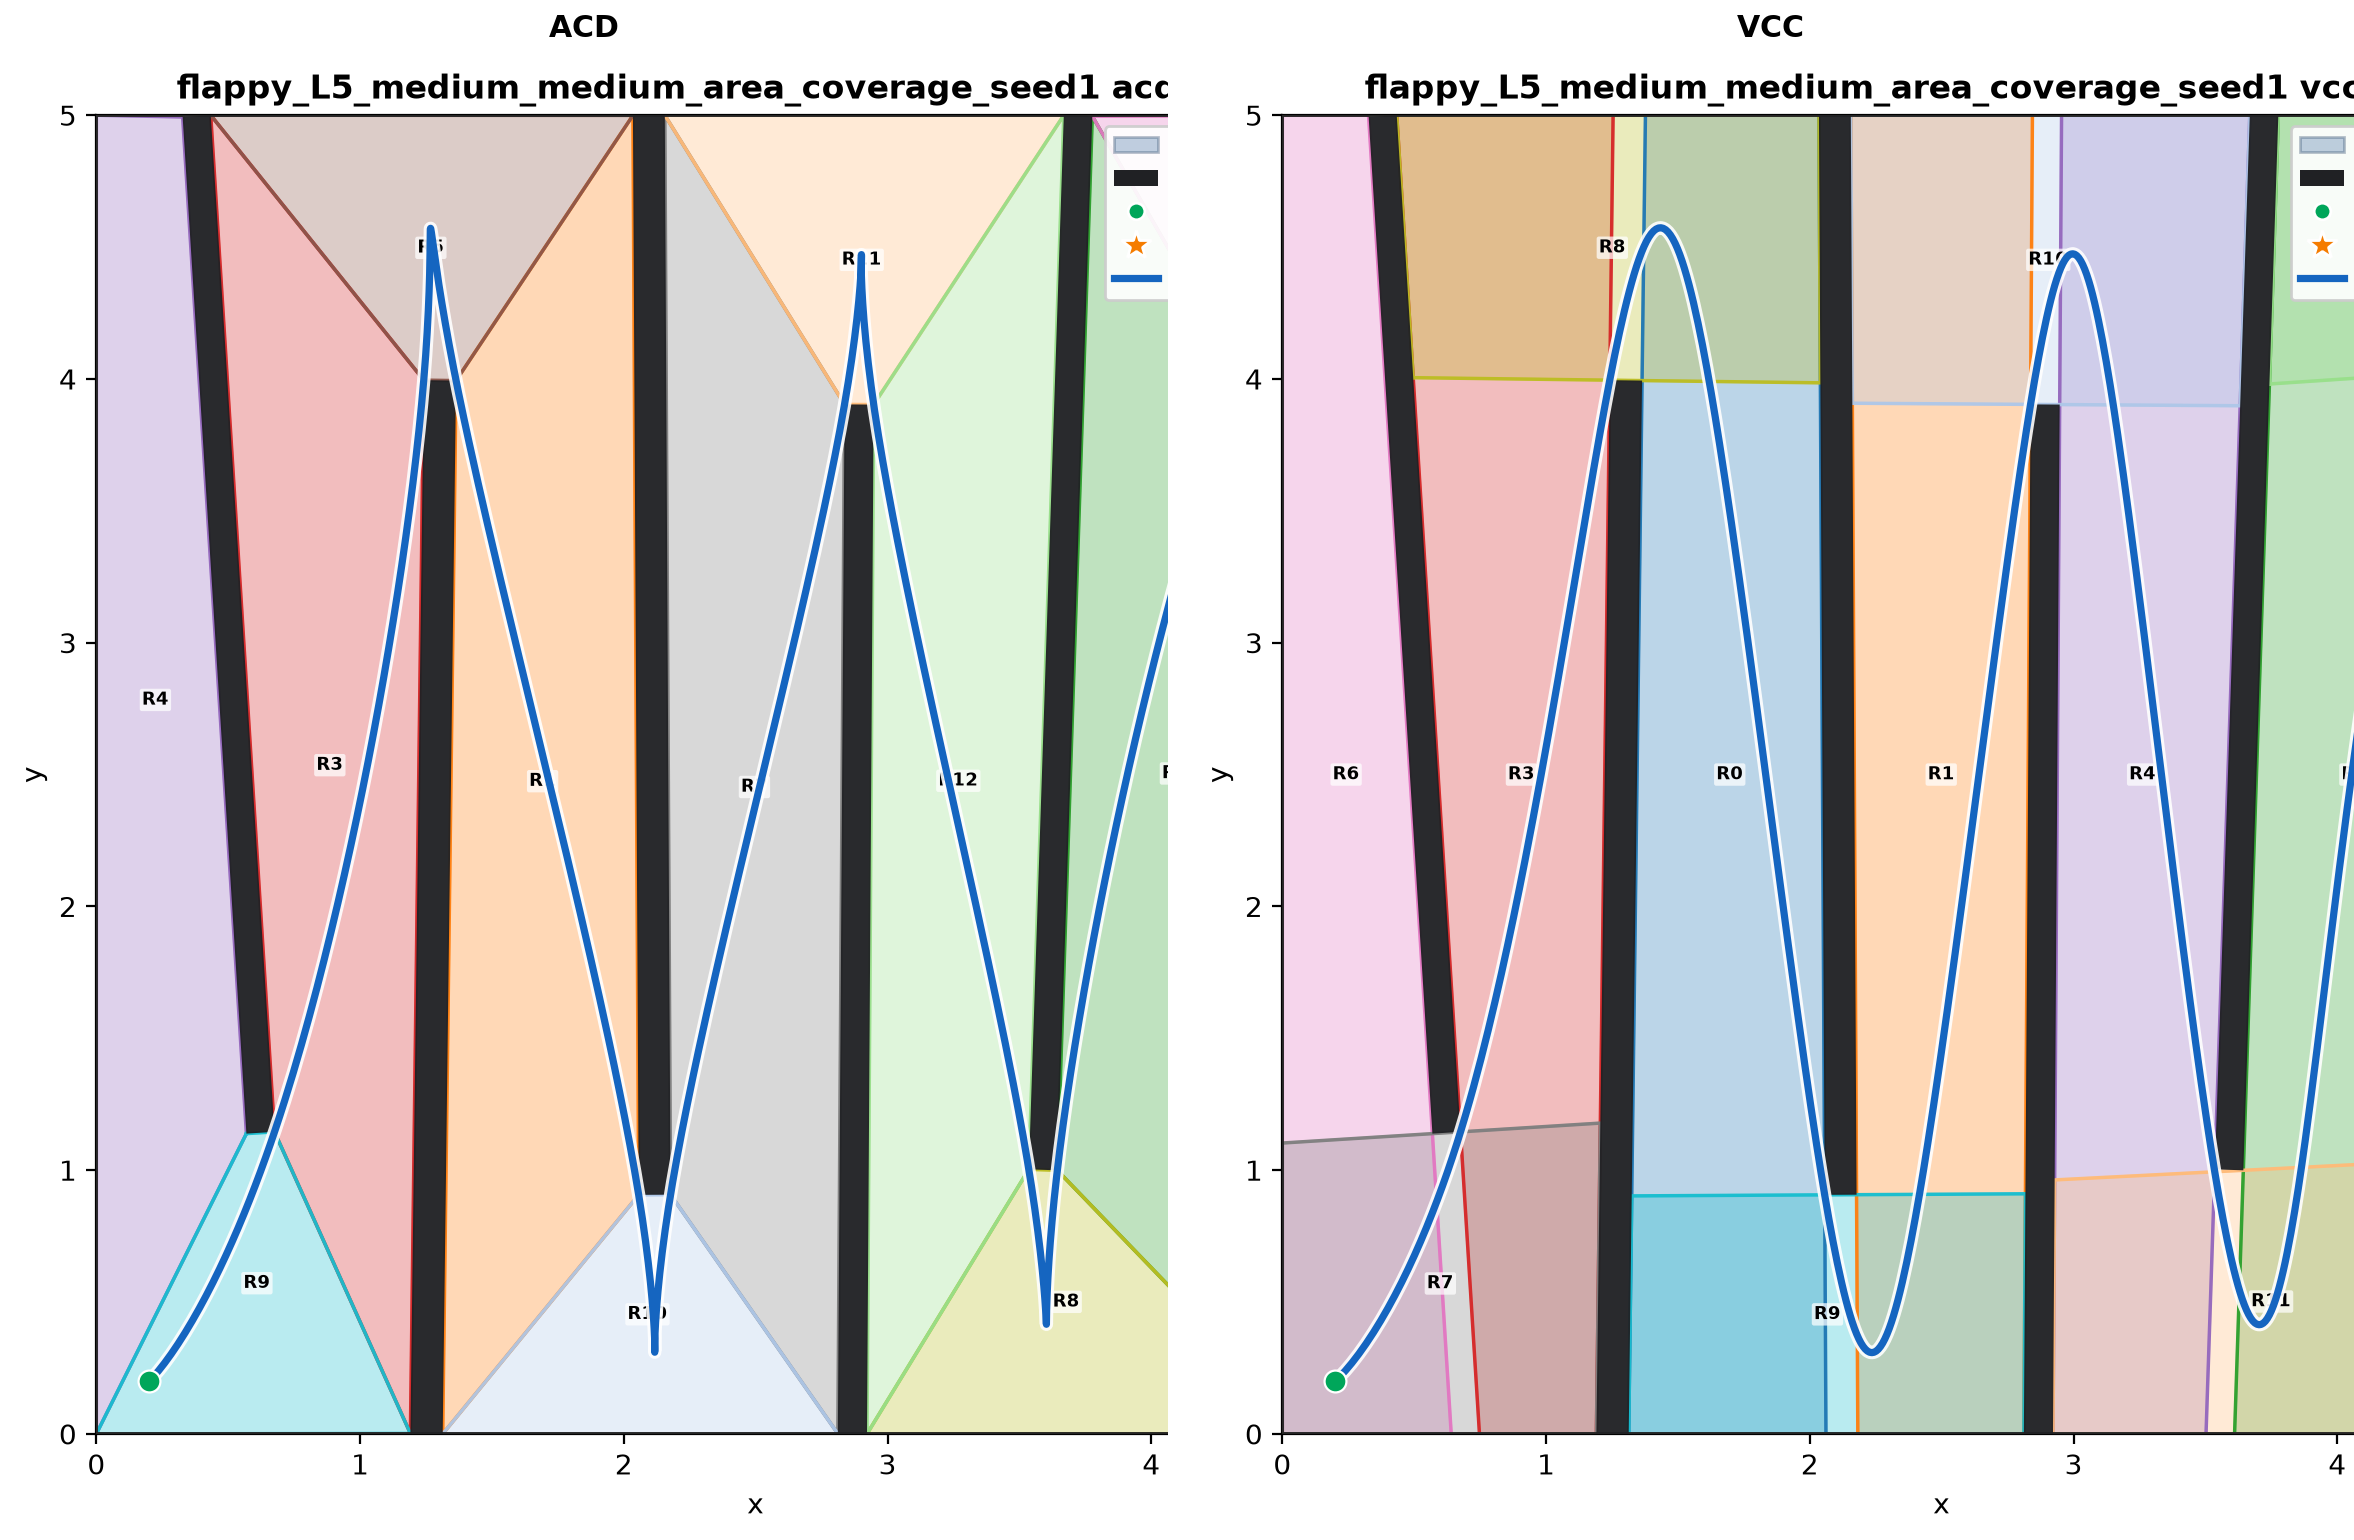
\includegraphics[width=0.48\textwidth]{5-Experimental-results/figures/flappy_seed1_comparison.png}
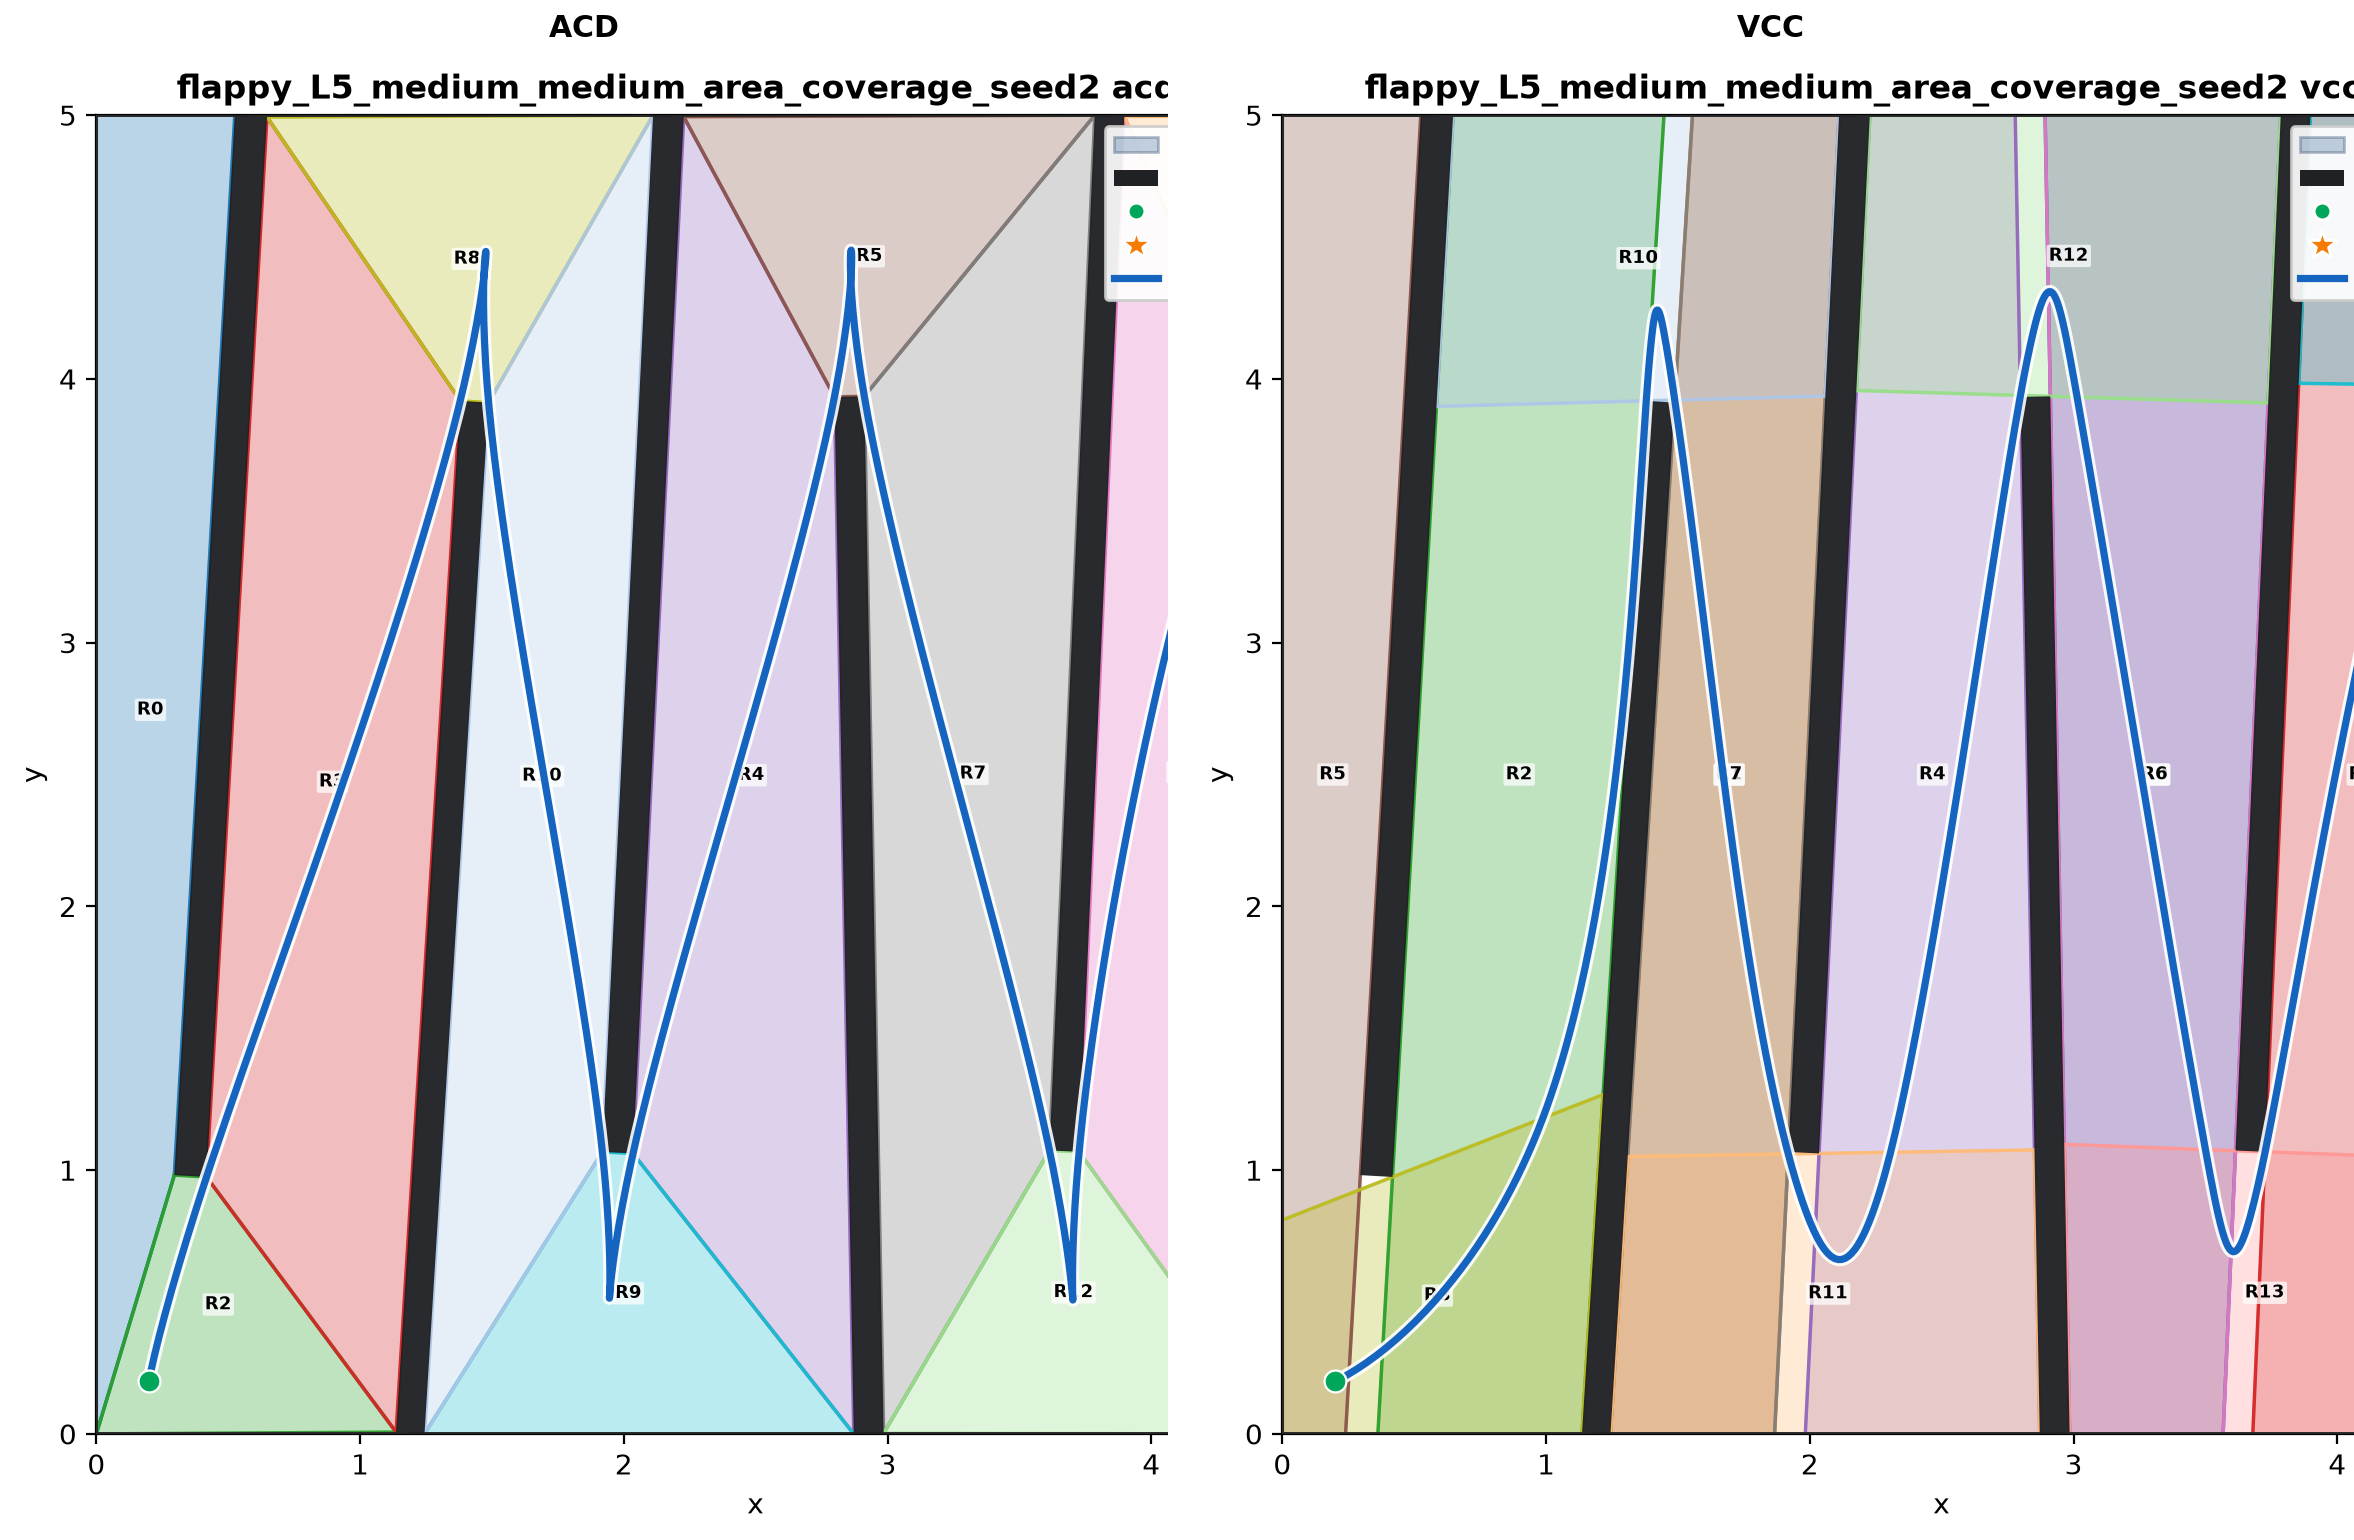
\includegraphics[width=0.48\textwidth]{5-Experimental-results/figures/flappy_seed2_comparison.png}
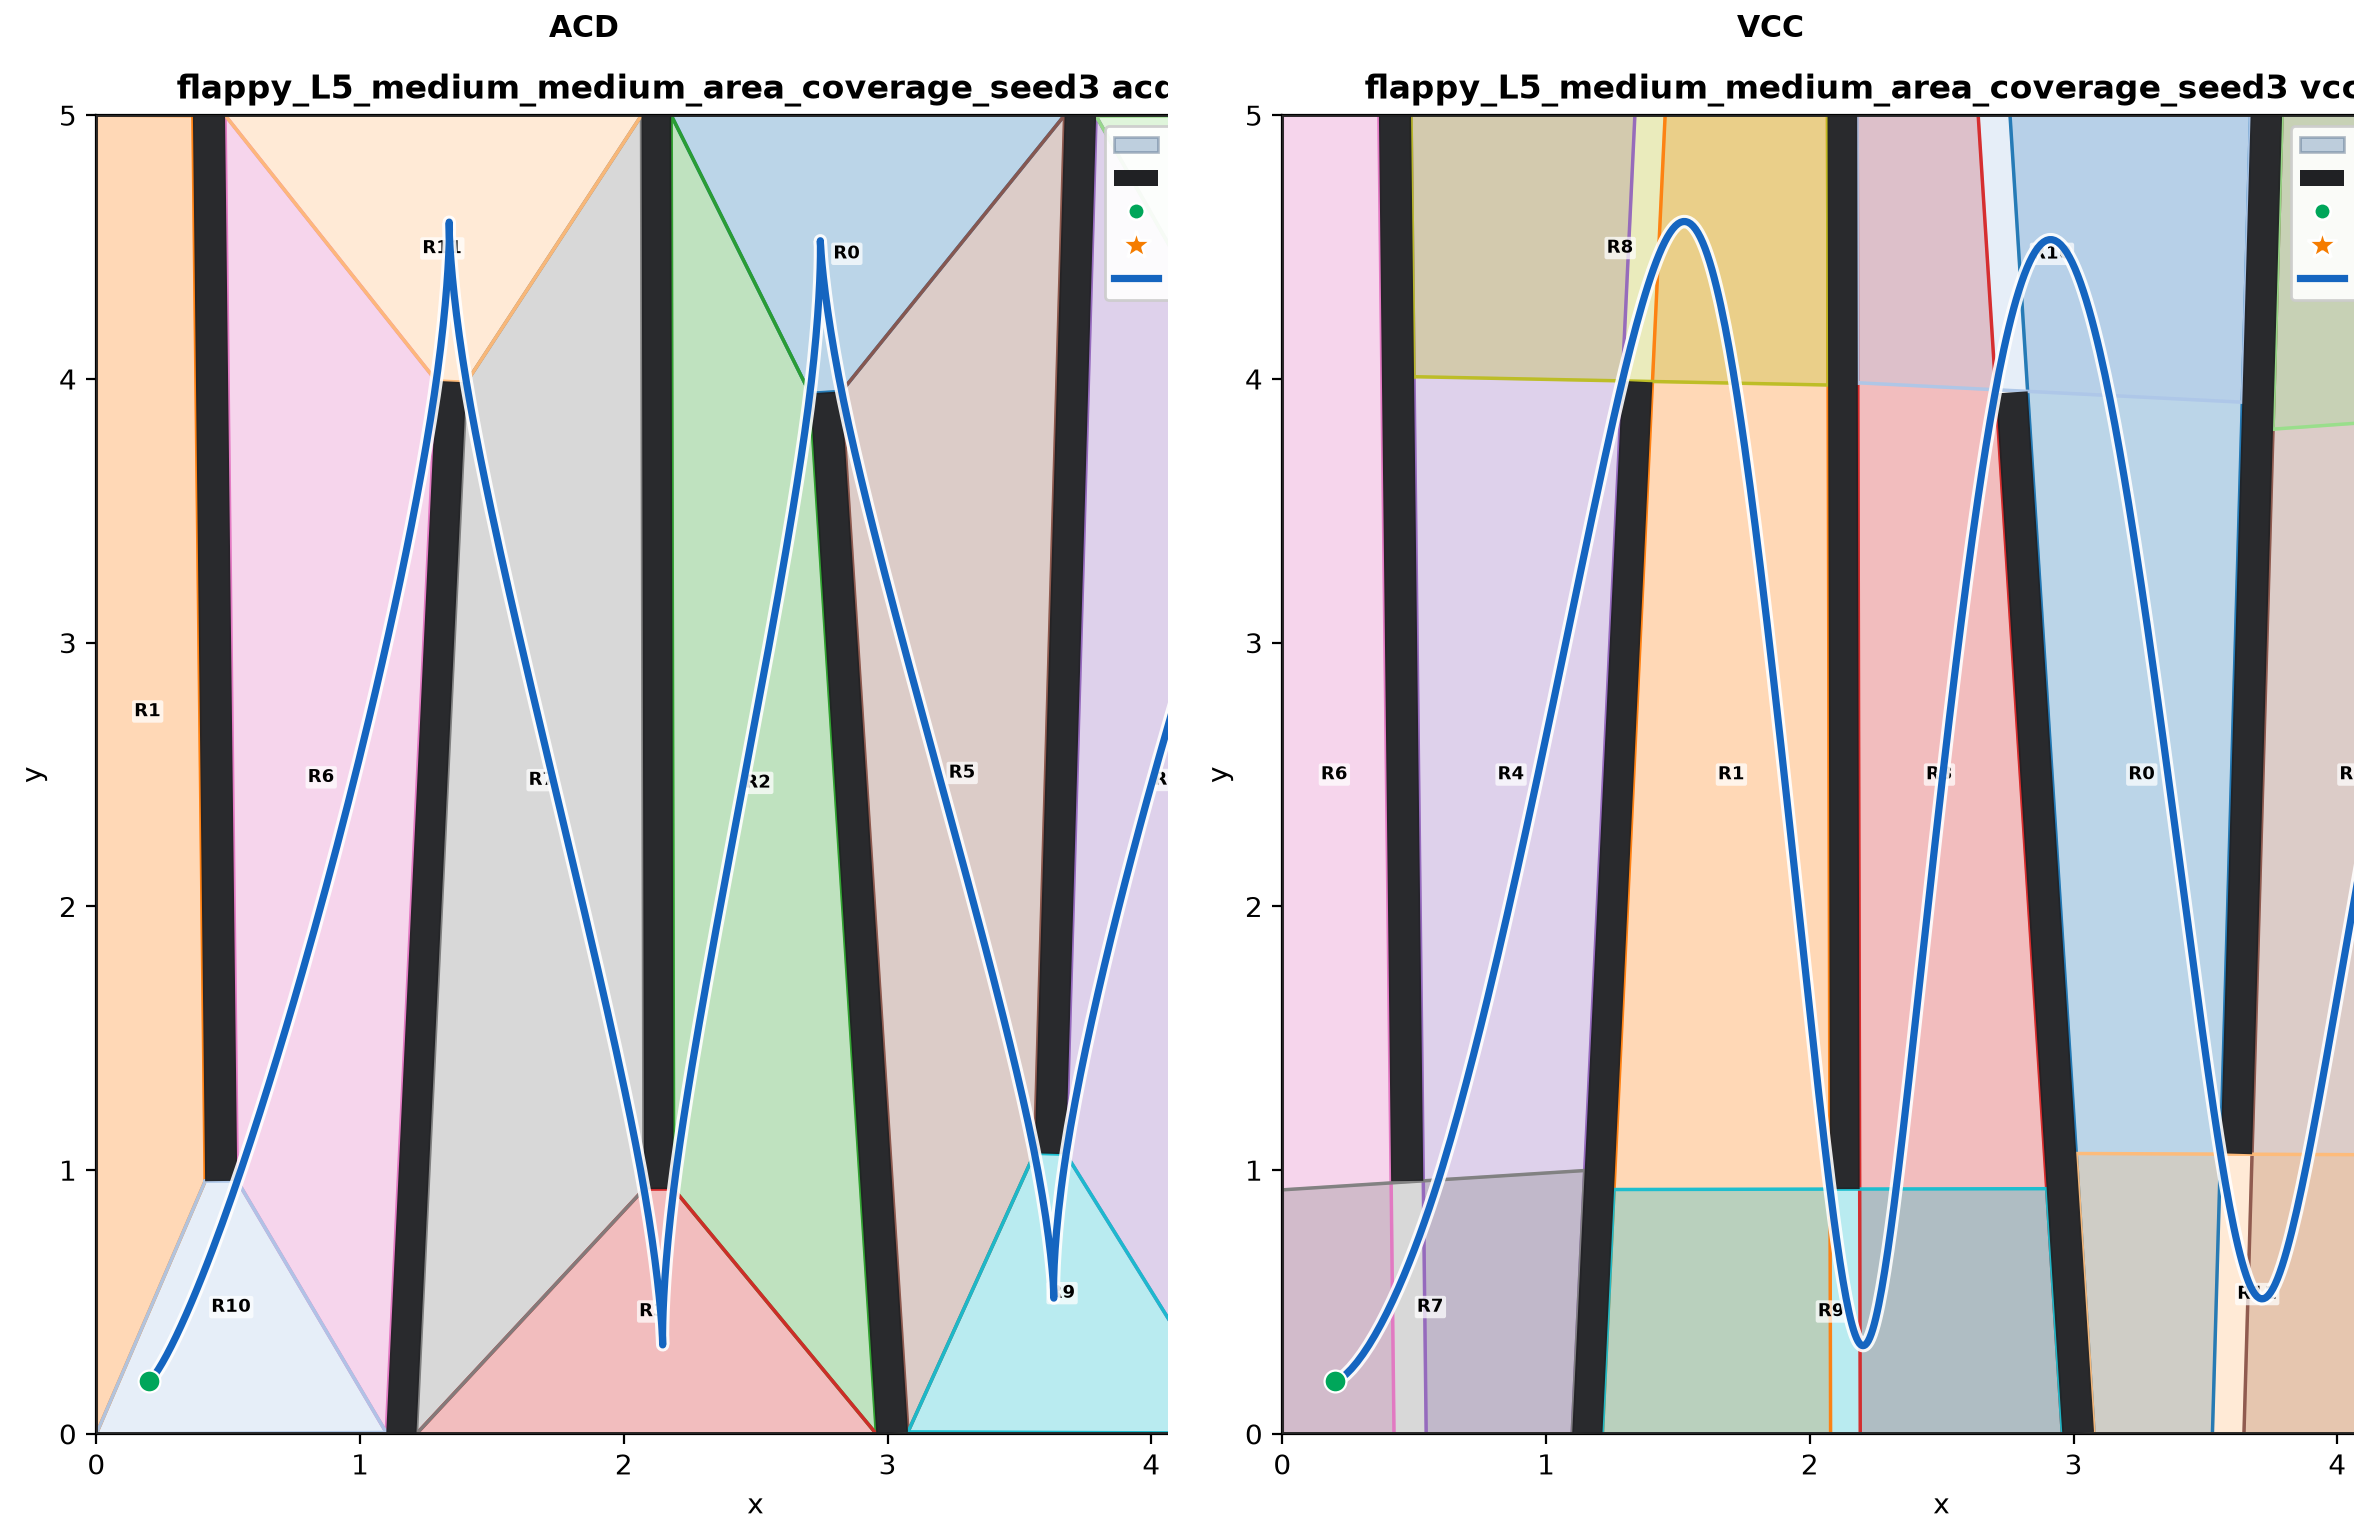
\includegraphics[width=0.48\textwidth]{5-Experimental-results/figures/flappy_seed3_comparison.png}
% 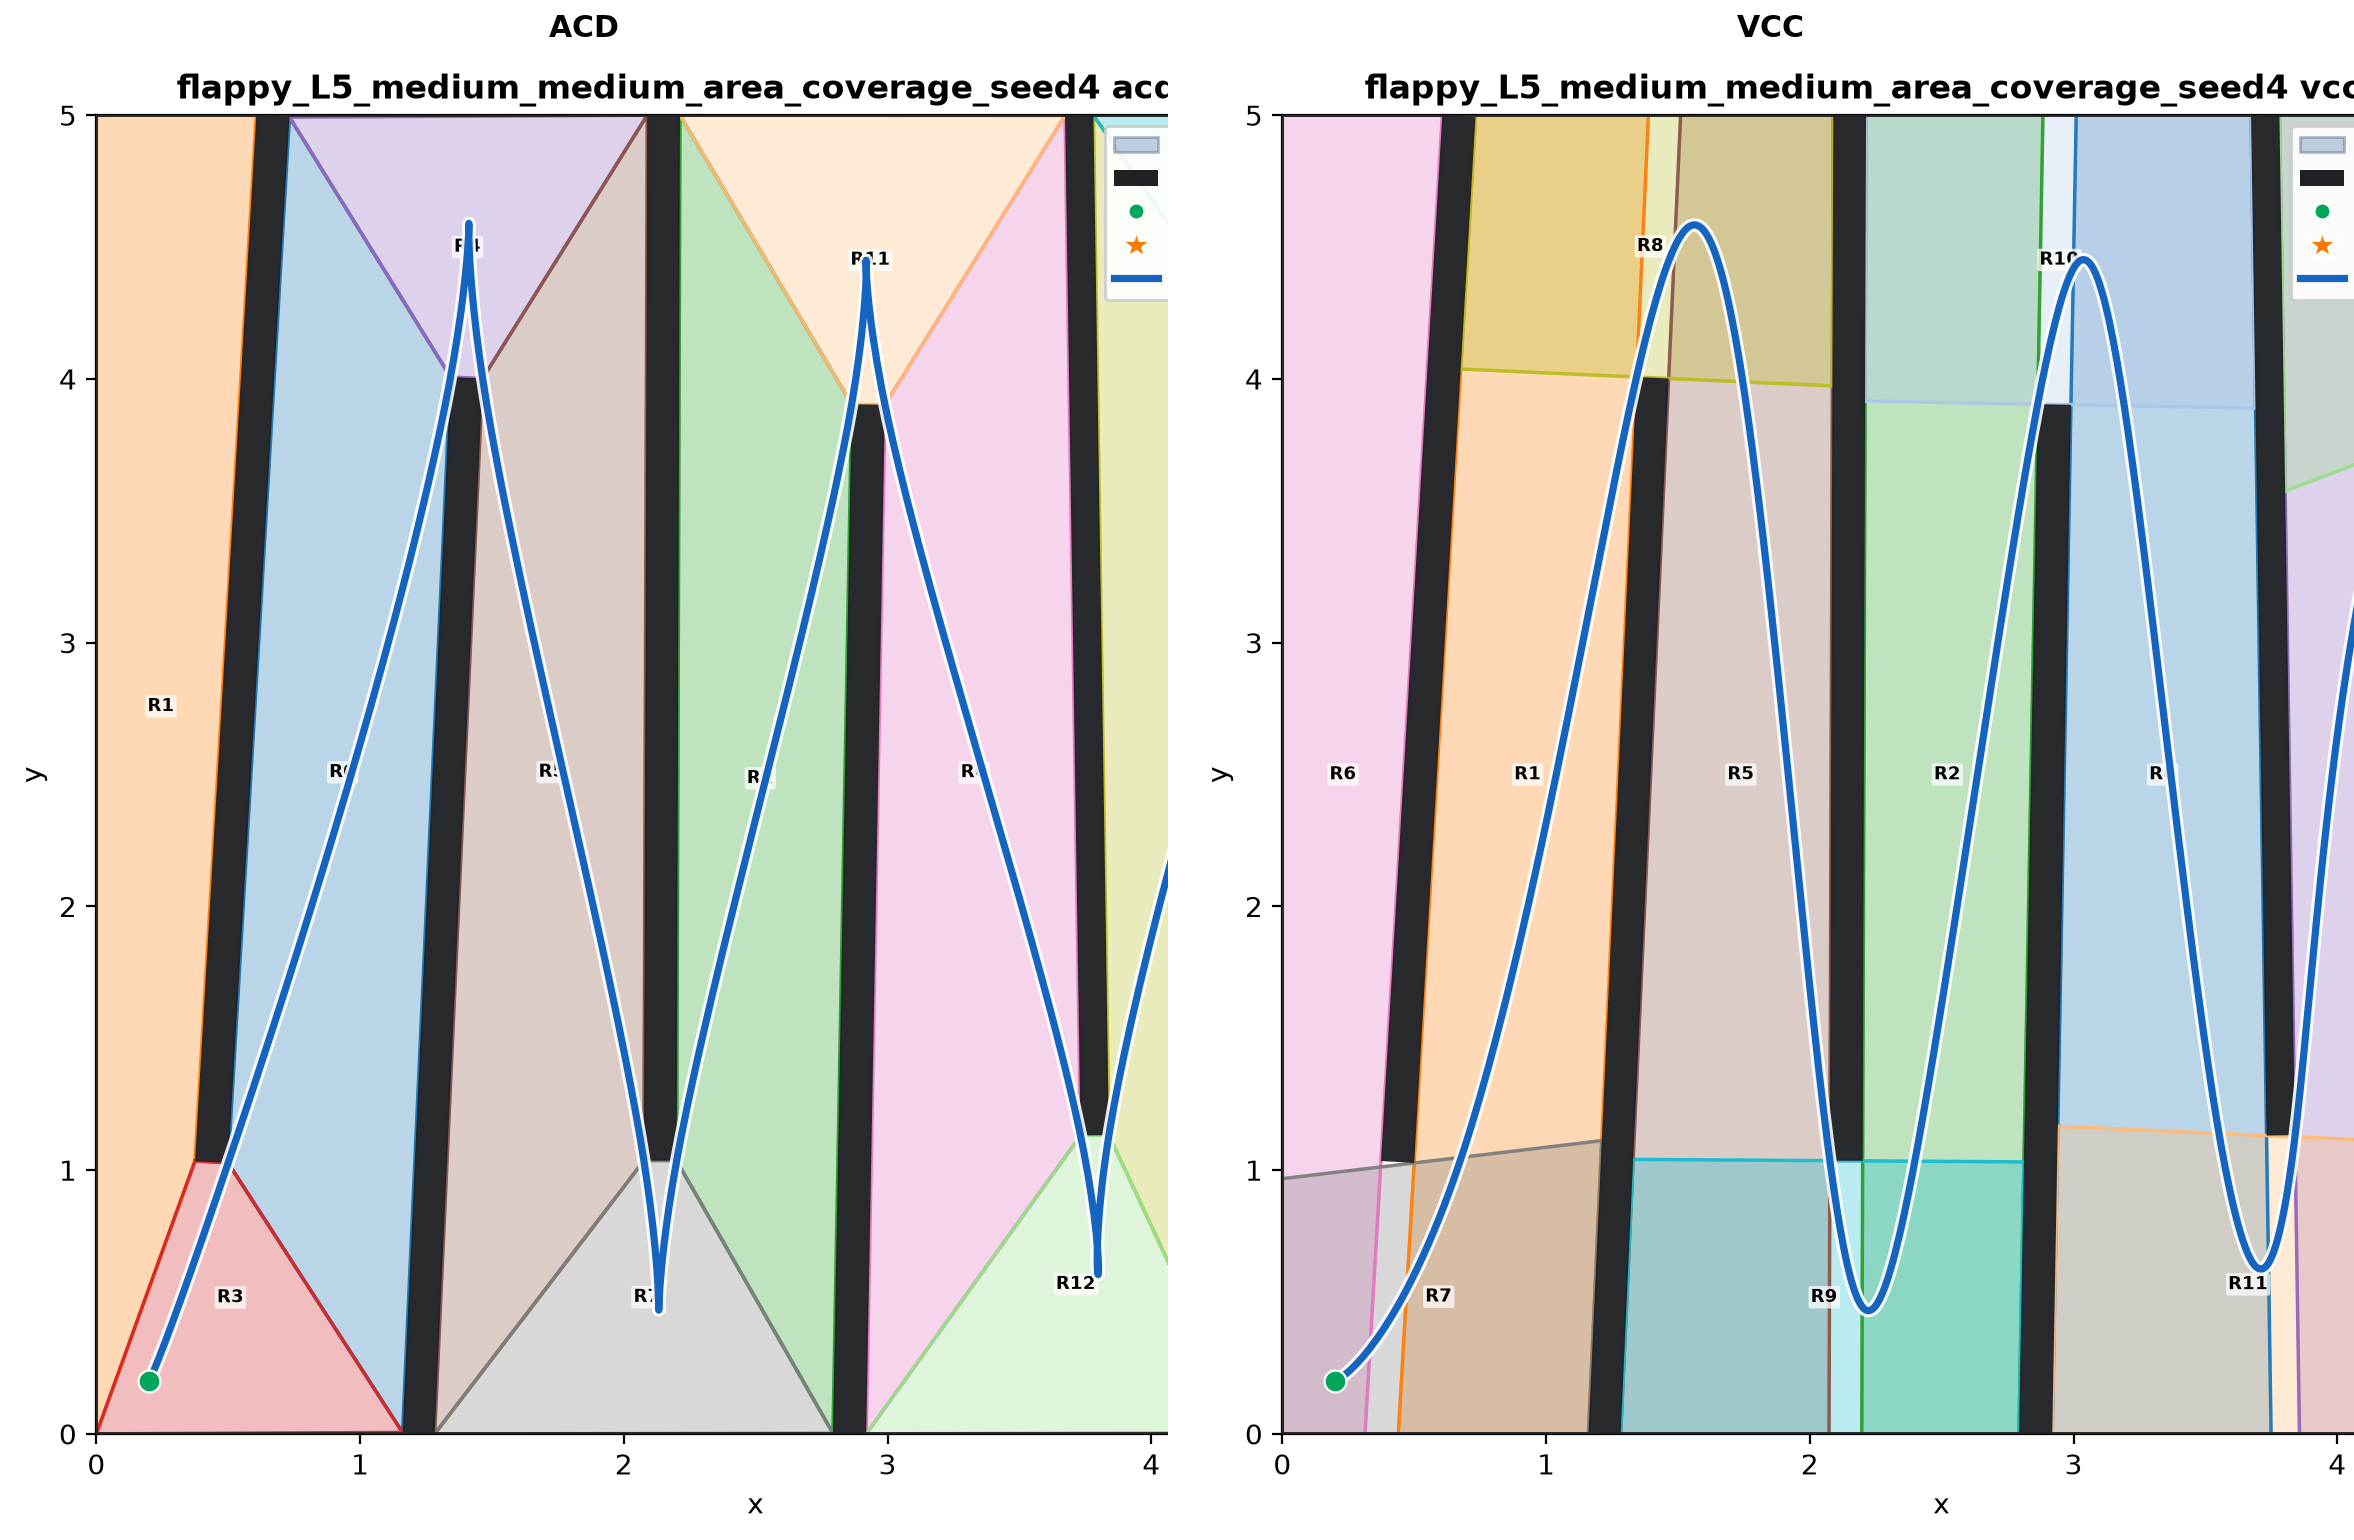
\includegraphics[width=0.48\textwidth]{5-Experimental-results/figures/flappy_seed4_comparison.png}
\caption{ACD and VCC comparisons on four representative \code{flappy} geometries. Obstacles are black, convex regions are colored, and the GCS trajectory is plotted in blue.}
\label{fig:exp-flappy}
\end{figure}

The principal difference is computational rather than geometric. ACD's median
end-to-end time is 2.08~s (IQR $[2.07,2.13]$~s), whereas VCC requires 21.87~s
(IQR $[21.75,22.19]$~s), almost entirely because of decomposition. Since both
methods induce the same median graph size ($N_R=25$, $N_E=24$), this family is
a controlled example in which VCC pays its sampling and clique-cover overhead
without obtaining a smaller online optimization problem.

\subsection{Discussion and Limitations}
The experiments identify the induced edge structure, rather than the number of
convex regions alone, as the most informative decomposition-level predictor of
GCS cost. VCC is advantageous online when visibility-based aggregation removes
both regions and adjacencies, as on \code{clustered} and \code{rooms}; it loses
that advantage when aggregation leaves a dense overlap graph, as on
\code{u\_shaped}, or leaves the graph essentially unchanged, as on
\code{flappy}. These results motivate reporting $N_E$, presolved program size,
relaxation and rounding behavior, and reliability alongside $N_R$.

The appropriate method consequently depends on query regime. For a single
start--goal query, ACD dominates end-to-end runtime in every tested family and
also achieves a 50/50 geometry success rate. VCC becomes attractive when the
environment decomposition is reusable: its one-time cost can be amortized over
multiple start--goal pairs, changes in trajectory boundary conditions, or
repeated replanning on a static map. If $t_{\rm dec}^{A}$ and
$t_{\rm dec}^{V}$ denote decomposition costs and $t_{\rm GCS}^{A}$ and
$t_{\rm GCS}^{V}$ denote per-query solve costs, VCC breaks even after
approximately
\(
Q^{\star}=(t_{\rm dec}^{V}-t_{\rm dec}^{A})/
(t_{\rm GCS}^{A}-t_{\rm GCS}^{V})
\)
queries whenever $t_{\rm GCS}^{A}>t_{\rm GCS}^{V}$. The family medians give
$Q^{\star}\approx2$ for \code{clustered} and $Q^{\star}\approx6$ for
\code{rooms}; no positive break-even point exists for families in which VCC
does not reduce per-query GCS time. This calculation assumes that the graph can
be reused without rebuilding and excludes any query-dependent preprocessing.

The clearance results expose a separate design trade-off. VCC often returns
trajectories with greater sampled minimum clearance, plausibly because larger
visibility cliques provide broader overlapping sets through which the
continuous trajectory can move. Achieving those sets requires extensive
visibility sampling and clique construction, however, and global coverage does
not ensure that every narrow gateway is represented robustly. A decomposition
selected for clearance may therefore incur both additional offline cost and
stochastic connectivity risk. Applications should treat coverage, graph
connectivity, and clearance as distinct acceptance criteria.

Several limitations bound these conclusions. First, the 50 geometries cover one
workspace scale, density level, obstacle-size level, VCC sample budget (500),
and coverage target (0.96). Second, the supplied summary CSVs retain quartiles
and population variance but omit trial-level certificate fields and failure
messages; consequently, the proposed narrow-gateway mechanism cannot be
verified without the raw logs. Third, the reported Wilcoxon tests operate on
geometry-level VCC medians to avoid pseudoreplication, but larger geometry sets
and paired bootstrap confidence intervals are needed for precise effect
estimation within each family. Finally, sampled minimum clearance is sensitive
to trajectory discretization and is not a continuous-time collision
certificate. Future experiments should vary sampling budget, target coverage,
workspace scale, and obstacle density; retain stage-resolved failures; evaluate
graph connectivity before optimization; and measure amortized performance over
explicit multi-query workloads.
